\section{VL vom 30.~November 2010}
Bereinigt sein: Jede Variable darf nur 1 mal auftauchen. (Umbenennen)
\subsection{Beispiel PNF}

\begin{align}
  \varphi &= \NOT\forall x.(R(x,x) \AND \forall x.\exists y.R.(x,y)) && \text{(Fall 3)} \\
    &\EQUIV \NOT\forall x.(R(x,x) \AND \forall z.\exists y.R.(z,y)) && \text{(Variablenumbenennung)} \\
    &\EQUIV \NOT\forall x.\forall z.\exists y.(R(x,x) \AND R(z,y)) && \text{(Negation reinziehen)} \\
    &\EQUIV \exists x.\exists z.\forall y. \NOT(R(x,x) \AND R(z,y))
\end{align}

\subsection{Postsches Korrespondenzproblem (PCP)}
Unentscheidbarkeit\\
\seeslide{57}

\[
  F = \set{(0,1)_1, (1,10)_2, (01,1)_3}
\]

Indexfolge 2,3 ist Lösung:

\begin{itemize}
  \item linke Konkatenation:  $1|0 1$
  \item rechte Konkatenation: $1 0|1$
\end{itemize}

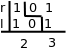
\includegraphics[width=3cm]{30_11_10_1.png}

\subsubsection{Unentscheidbarkeit}

\begin{verbatim}
  Baum von Carsten TikZen
\end{verbatim}

\subsubsection{Beweis des Lemmas Unentscheidbarkeit}

\begin{description}
  \item[\enquote{$\Leftarrow$}]
  Sei $\varphi_F$ fültig. Betrachte folgende Struktur:
  \begin{align*}
    \Afrak &= (A, c_\epsilon, f_0, f_1, P) \qquad\text{mit} \\
    A &= \set{0,1}^*\\
    c_\epsilon^{\Afrak} &= \epsilon\\
    f_0^{\Afrak}(w) &= w \cdot 0\\
    f_1^{\Afrak}(w) &= w \cdot 1\\
    P &= \set{(u,v) \mid \text{es gibt $i_1,\dots,i_l$ mit $u=u_{i_1}\cdots u_{i_l}$ und $v=v_{i_1}\cdots v_{i_l}$}}
  \end{align*}
  
  Es gilt
  \begin{enumerate}
    \item $\Afrak \models \varphi$ (nach Definition von $P$ und wegen
    $t_w(c_\epsilon)^{\Afrak}=w$ für alle $w\in\set{0,1}^*$)
    
    \item $\Afrak \models \psi$: wenn $(u,v)\in P^{\Afrak}$, dann folgt
    mit Definition von $P$ auch $P(uu_i, vv_i)$ für $1\leq i\leq h$.
    
    Wegen $t_w^\Afrak(w') = w'w$ für alle $w,w'\in\set{0,1}^*$, also
    $P(t_{u_i}^\Afrak(u), t_{v_i}^\Afrak(v))$.

    Wegen Gültigkeit von $\varphi_F$, also $\Afrak \models \exists
    x.P(x,x)$. Nach Definition von $P$ hat $F$ aleo eine Lösung.
  \end{enumerate}
  
  \item[\enquote{$\Rightarrow$}]
  Sei $i_1,\dots,i_l$ Lösung für $F$ und $\Afrak = (A, c, f_1, f_2, P)$
  eine Struktur. Zu zeigen: $\Afrak\models\varphi_F$.
  
  Wenn $\Afrak\not\models \varphi\AND\psi$, gilt $\Afrak\models\varphi_F$.
  Es gelte $\Afrak\models\varphi\AND\psi$. Definiere Abbildung $h:\set{0,1}^*
  \rightarrow A$:
  \begin{align*}
    h(\epsilon) &= c_\epsilon^\Afrak\\
    h(w0) &= f_0^{\Afrak}(h(w))\\
    h(w1) &= f_1^{\Afrak}(h(w))
  \end{align*}
  
  Man sieht leicht, dass $h(w)=t_w(c_\epsilon)^\Afrak$ für alle $w\in\set{0,1}^*$.
  
  Wegen $\Afrak \models \varphi$, also $(h(u_{i_1}), h(v_{i_1}) \in P^{\Afrak}$.
  
  Wegen $\Afrak \models \psi$ können wir unduktiv schließen, dass
  $(h(u_{i_1}\cdots u_{i_r}), h(v_{i_1}\cdots v_{i_r}))\in P^{\Afrak}$
  für $1\leq r\leq l$.
  
  Sei $u_{i_1}\cdots u_{i_r} = v_{i_1}\cdots v_{i_r} = w$. Es gilt also
  $(h(w),h(w)) \in P^{\Afrak}$, damit $\Afrak \models \exists x.P(x,x)$,
  also $\Afrak\models\varphi_F$.
\end{description}

Gleichheit nicht wichtig für Entscheidbarkeit.\\
\seeslide{60}

\subsection{Beweis Theorem}

Wir nehmen o.B.d.A. an, dass $\varphi$ ein Satz ist (universeller Abschluss).

\begin{description}
  \item[\enquote{$\Leftarrow$}]
  Angenommen, $\varphi$ ist nicht gültig. Dann gibt es Struktur $\Afrak$
  mit $\Afrak\not\models\varphi$. Erweitere $\Afrak$ um $P^\Afrak =
  \set{(a,a)\mid a\in A}$.
  
  Offensichtlich gilt $\Afrak\models\ANDop\Gamma_\tau$. Man zeigt leicht,
  dass $\Afrak,\beta\models\psi$ gdw. $\Afrak,\beta\models\psi[P_=/=]$ für
  alle $\psi\in FO(\tau)$ und Zuweisungen $\beta$. Wegen
  $\Afrak\not\models\varphi$, also $\Afrak\not\models\varphi[P_=/=]$, also
  $\Afrak\not\models\ANDop\Gamma_\tau \rightarrow \varphi[P_=/=]$, damit
  ist diese Formel nicht gültig.
  
  \item[\enquote{$\Rightarrow$}]
  Angenommen, $\ANDop\Gamma_\tau \rightarrow \varphi[P_=/=]$ ist nicht
  gültig. Dann gibt es Struktur $\Afrak$ mit $\Afrak\not\models\ANDop
  \Gamma_\tau\rightarrow\varphi[P_=/=]$. Dann $\Afrak\models\ANDop
  \Gamma_\tau$ und $\Afrak\not\models\varphi[P_=/=]$. Wegen ersterem ist
  $P_=^\Afrak$ Äquivalenzrelation auf $A$. Für $a\in A$ sei $[a]$ die
  Äquivalenzklasse von $a$. Definiere Struktur $\hat{\Afrak}$
  (Quotientenstruktur):
  
  \begin{align*}
    \hat{A} &= \set{[a] \mid a\in A}\\
    R^{\hat{\Afrak}} &= \set{([a_1],\dots,[a_n]) \mid (a_1,\dots,a_n) \in R^\Afrak }\\
  \end{align*}
  \seeslide{63}
  Für jede Zuweisung $\beta$ in $\Afrak$ sei $\hat{\beta}$ die
  Zuweisungen in $\hat{\Afrak}$ mit $\hat{\beta}(x)=[\beta(x)]$. Man
  zeigt per Induktion über die Struktur von $\psi$
  
  \begin{itemize}
    \item[$(*)$] Für alle $\psi\in FO(\tau)$ und alle Zuweisungen $\beta$
    gilt $\Afrak,\beta\models\psi[P_=/=]$ gdw. $\hat{\Afrak},\hat{\beta}\models\psi$.
  \end{itemize}
  
  Wegen $\Afrak\not\models\varphi[P_=/=]$ folgt $\hat{\Afrak}\not\models\varphi$, also ist $\varphi$ nicht gültig.
\end{description}
\qed

Es gibt unendl. Modell erfüllbar, dass bei endl. Modell nicht erfüllbar ist.\\
Domänenabhängigkeit wichtig.\\
\seeslide{62}
Zu welchem Problem in der Logik erster Stufe korrespondieren?\\
- Erfüllbarkeit

Unendliche Menge von Formeln gesehen bei Kompaktheitstheorem. Unter Konsequenz abgeschlossen,
wenn $\varphi$ aus T folgt, muss $\varphi$ bereits in T drin sein.
